\documentclass[parskip=full]{scrartcl}
\setcounter{tocdepth}{2}
\usepackage[T1]{fontenc}    % avoid garbled Unicode text in pdf
\usepackage[utf8]{inputenc} % use utf8 file encoding for TeX sources
\usepackage[german]{babel}  % german hyphenation, quotes, etc
\usepackage{hyperref}       % detailed hyperlink/pdf configuration
\hypersetup{                % ‘texdoc hyperref‘ for options
pdftitle={PSE: Entwicklung eines relationalen Debuggers - Testbericht},%
,%
}
\usepackage{graphicx}       % provides commands for including figures
\usepackage{csquotes}       % provides \enquote{} macro for "quotes"
\usepackage[nonumberlist]{glossaries}     % provides glossary commands
\usepackage{enumitem}
\usepackage{pdfpages}
\usepackage{xcolor}
\newcommand\frage[1]{\textcolor{red}{#1}}
\renewcommand{\glstextformat}[1]{\textbf{\color{blue}\em #1}}

\newglossaryentry{Komponententest}
{
    name={Komponententest},
    plural={Komponententests},
    description={
        Ein Komponententest ist ein Test eines Softwaresystems, der eine Komponente des Systems testet.
        Beim Durchführen eines Komponententests einer Komponente werden keine anderen Komponenten verwendet.
        Als Komponente sei in diesem Kontext ein Paket oder eine Klasse bezeichnet.
    }                
}

\newglossaryentry{Testhelfer}
{
    name={Testhelfer},
    plural={Testhelfern},
    description={
        Ein Testhelfer ist ein Programmteil der zur Durchführung von Tests eines Softwaresystems verwendet wird.
        Der Testhelfer soll als Platzhalter oder Stellvertreter für andere Systemkomponenten des Systems dienen.
    }                
}

\makeglossaries

\font\myfont=cmr12 at 20pt

\title{
	\vspace{2cm}
	\myfont 
	Praxis der Softwareentwicklung:\\ 
	Entwicklung eines relationalen Debuggers\\
}
\subtitle{
	\vspace{1cm}
	\myfont
	Testbericht
}

\author{
	\vspace{1cm} \\
	Benedikt Wagner\\
	\and 
        \vspace{1cm} \\ 
        Chiara Staudenmaier\\
        \and 
        \vspace{1cm} \\
        Etienne Brunner\\
	\and Joana Plewnia\\
	\and Pascal Zwick\\
	\and Ulla Scheler\\
	\vspace{1cm}
	\and Betreuer: Mihai Herda, Michael Kirsten
	\vspace{4cm}
}

\begin{document}
\clearpage
\maketitle
\pagenumbering{gobble}
\newpage

\tableofcontents
\newpage
\pagenumbering{arabic}

\section{Übersicht}

\subsection{Einleitung}
%Einleitung mit grobem Überblick. Dieser Abschnitt soll an das Pflichtenheft anschließen.
Dieses Dokument dokumentiert die Ergebnisse der Qualitätssicherungsphase (\textit{19,02.-12.03.2018}) im Rahmen des Moduls Praxis der Softwareentwicklung (PSE) am Lehrstuhl \enquote{Anwendungsorientierte formale Verifikation - Prof. Dr. Beckert} am Karlsruher Institut für Technologie (KIT).\\
Hierbei handelt es sich um die Qualitätssicherung des \textit{DIbuggers}, der im Pflichtenheft definiert und in folgenden Dokumenten entworfen und implementiert wurde. Aufgabe des \textit{DIbuggers} ist es, dem Nutzer zu helfen, mehrere Programme gleichzeitig zu debuggen und interaktiv zu analysieren. \\

\begin{figure}[!h]
\centering

\includegraphics[width=0.6\textwidth]{../Plichtenheft/logo_nongi.png}
\caption{Produktlogo}
\end{figure}

\subsection{Kurzer Überblick über den Entwurf}
An dieser Stelle soll der Entwurf des \textit{DIbuggers} noch einmal kurz erläutert werden, da in folgenden Abschnitten darauf Bezug genommen wird. Eine weitere Übersicht bietet Abbildung \ref{Architekturdiagramm}. Für detailliertere Informationen sei der Leser auf das Entwurfsdokument verwiesen.

\begin{figure}[!h]
\centering
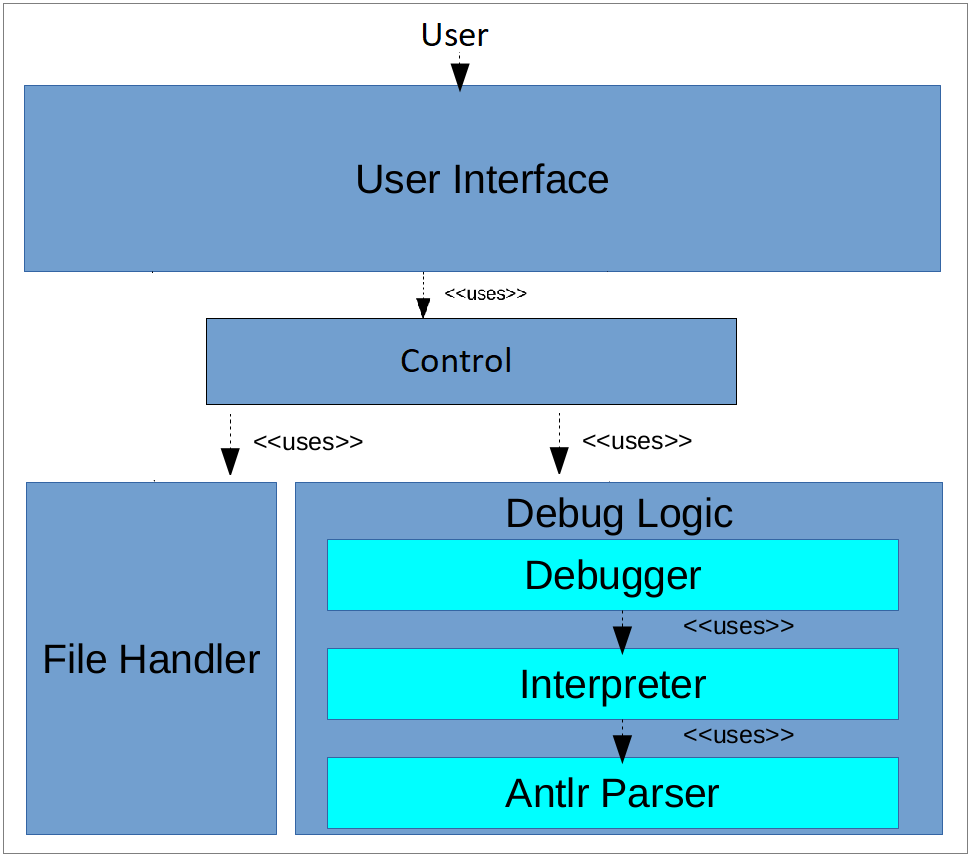
\includegraphics[width=0.5\textwidth]{../Plichtenheft/Architektur.png} \\
\caption{Architekturdiagramm}
\label{Architekturdiagramm}
\end{figure}
Die Architektur des \textit{DIbuggers} orientiert sich am Model-View-
-Entwurfsmuster und beinhaltet ein weiteres Paket zum Umgang mit Dateien. Das Produkt ist entsprechend aufgeteilt in die vier Pakete \textit{DebugLogic} (Model), \textit{UserInterface} (View),  \textit{Control} (Control) und \textit{FileHandler}. 
Dabei hat jedes Paket seine eigene Aufgabe:
\begin{itemize}
\item Die \textit{DebugLogic} enthält die Anwendungslogik.
\item Das \textit{UserInterface} beinhaltet den Code für die Benutzeroberfläche, also alles, was der Nutzer vom Produkt sieht.
\item Die \textit{Control} nimmt die Benutzereingaben entgegen und steuert die Interaktion zwischen dem \textit{UserInterface} und der \textit{DebugLogic}.
\item Der \textit{FileHandler} ist dazu da, Daten zu speichern und zu lesen.
\end{itemize}


\subsection{Erklären des Vorgehens}
Zunächst wurden alle Pakete abgesehen von der Benutzeroberfläche Paket-/Klassenweise auf Fehler getestet (siehe Abschnitt \ref{einzelnePakete}).
Die Grundfunktionalität der Benutzeroberfläche wurde in nicht-automatisierten Tests erprobt (siehe Abschnitt \ref{gui}) und orientierte sich dabei an den im Pflichtenheft definierten Testfällen. Im Pflichtenheft geforderte nicht-funktionale Anforderungen an die Benutzeroberfläche, wie zum Beispiel Verständlichkeit und Erlernbarkeit, wurden mittels eines Nutzertestes gesondert erhoben (siehe Abschnitt \ref{usertestimdoc}).
Die Fehlertoleranz und Stabilität des Systems wurde hauptsächlich mit Hilfe von Unit-Tests getestet. Da viele unzulässige Nutzereingaben bereits auf Ebene des Interpreterpakets getestet wurden, fällt die Zahl der entsprechenden Belastungstests (siehe Abschnitt \ref{stress}) geringer aus. Untersuchungen zu verschiedener Hard- und Software, sowie Laufzeit und Speicherverbrauch, finden sich ebenfalls in Abschnitt \ref{gesamthwsw} .

\newpage
\section{Testen einzelner Pakete}\label{einzelnePakete}

\subsection{Gesamtabdeckung}\label{abdeckung}
\begin{figure}[!h]
\centering
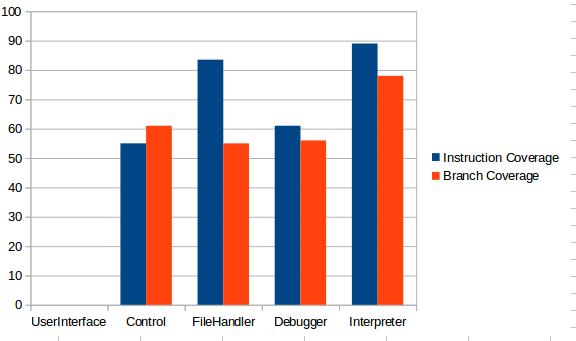
\includegraphics[width=1\textwidth]{paketeCoverage.png}
\caption{Testüberdeckung der Pakete}\label{AbdeckungPakete}
\end{figure}

In Abbildung \ref{AbdeckungPakete} ist die durch JUnit Tests erreichte Anweisungs und Zweigüberdeckung (mittels Eclemma ermittelt) dargestellt. Zu erwähnen ist, dass das User Interface, wie in \ref{gui} erklärt, nicht durch automatisierte Unittests überprüft wurde, sondern durch einen anderweitig ausgearbeiteten Testplan. Die hohe Abdeckung im Interpreter zeigt, dass dieser Teil ausgiebig getestet wurde und im Vergleich zu den anderen Paketen, wie etwa dem Debuggerpaket oder dem Paket \textit{Control}, prozentual gesehen weniger deligierende Methoden und getter und setter aufweist. \\
Die Gesamtabdeckung nach Klassen aufgeschlüsselt ist dem Archiv im SVN zu entnehmen.
Im Archiv sind Zeilen-, Anweisungs-, Zweig- und Klassenüberdeckung auf Paket- und/oder Klassenebene dokumentiert.
Nicht beinhaltet sind Angaben über die Abdeckung der Benutzeroberfläche mittels der in \ref{gui} beschriebenen Tests.
\subsection{AnltrParser}\label{ANTLRPARSER}
Das Paket \textit{AntlrParser} besteht lediglich aus von dem verwendeten Tool Antlr (siehe Entwurfsdokument Abschnitt 10.2) generierten Klassen. Da dieses Tool öffentlich bekannt und verbreitet ist, wurde es nicht explizit getestet. Die Korrektheit der von uns spezifizierten Grammatik, aus denen Antlr diese Klassen generiert, wurde im Rahmen der Tests des Paketes \textit{Interpreter} implizit getestet.
\subsection{Interpreter}
Im Interpreter wurden zunächst die Klassen der im Folgenden beschriebenen Reihenfolge für sich getestet. 
Dabei wurden die wichtigsten Methoden der Klassen zunächst so durch Unit-Tests getestet, dass eine möglichst hohe Testüberdeckung erreicht wurde. Die resultierende Überdeckung ist in Abbildung \ref{AbdeckungImInterpreter} dargestellt. Hierbei ist zu beachten, dass die mit \enquote{(av.)} gekennzeichneten abstrakten Klassen, mit dem Durchschnitt der jeweiligen Überdeckung ihrer Subklassen aufgeführt werden. \\ Zu beachten ist hierbei, dass die Termklassen eine Zweigüberdeckung von 100\% haben, was dadurch zu begründen ist, dass diese lediglich an andere Terme oder das Typsystem weiterdelegieren. So konnte die Entwurfsentscheidung des Kompositums hier eine gute Testbarkeit verursachen.
\begin{figure}[!h]
\centering
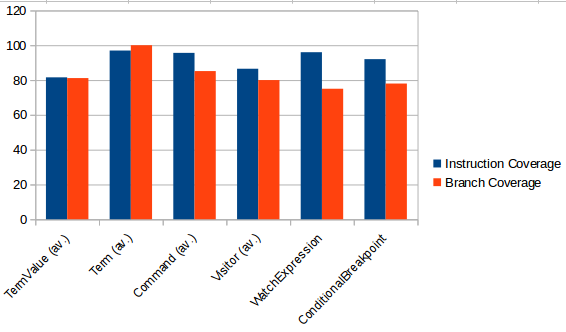
\includegraphics[width=0.8\textwidth]{interpreterCoverage.png}
\caption{Testüberdeckung der Teile des Interpreters}\label{AbdeckungImInterpreter}
\end{figure}


\subsubsection{Testen der Interpreterklassen}
Die Aufgabe des Interpreters ist das Ausführen der vom Nutzer als Quelltext gegebenen Programme. Hierzu wird zunächst der Quelltext vom in \ref{ANTLRPARSER} erklärten Paket in einen Syntaxbaum überführt.
Zwei im Interpreterpaket angesiedelte \textit{Visitor}-Klassen übersetzen diesen in einen Baum aus \textit{Commandobjekten}. Diese Objekte nutzen wiederum \textit{Terme} und diese nutzen, sobald sie ausgewertet werden, \textit{TermValues}, die das Typsystem der Wlang-Sprache darstellen. 
Da Commandklassen die Funktionsfähigkeit von Termen vorraussetzen und diese ein korrekt implementiertes Typsystem erfordern wurde dies hier in der Reihenfolge des Schreibens der Unittests berücksichtigt.
So wurden zunächst Unittest für die Implementierungen der abstrakten Klasse \textit{TermValue} geschrieben:
\paragraph{Testen der TermValues}
Um das Typsystem zu testen, wurden für jede Kombination von Datentypen (\texttt{char, int, long ... }) und jeden arithmetischen Operator (\texttt{+,-,\%,...}) sowie logischen und vergleichenden Operator(\texttt{<,>,!=,...}) Beispielwerte ausprobiert und mit dem korrekten Ergebnis verglichen. Hierbei fiel lediglich in der Klasse \textit{LongValue} ein Fehler auf (siehe \ref{fehlerImInterpreter}).\\
(siehe \textit{test.debuglogic.interpreter.TermValueTest.java})
\paragraph{Testen der Terme}
Bei den Termen wurde getestet, ob die konkrete Termausprägung (z.B. \textit{AdditionTerm}) bei Ausführen ihrer \textit{evaluate}-Methode das richtige Ergebnis liefert. \\
Da die Implementierung aufgrund des Entwurfs im Wesentlichen die Methoden der TermValues nutzt, wurde hier nicht mehr jede mögliche Datentypkombination getestet.\\
Hierbei fiel bei der Klasse \textit{ArrayAccessRelationalTerm} ein Fehler auf, der ebenfalls in \ref{fehlerImInterpreter} beschrieben ist. \\
(siehe \textit{test.debuglogic.interpreter.TermTest.java})
\paragraph{Testen der Commands}
Um die Commands zu testen, die einzelne Anweisungen oder Kontrollstrukturen in WLang-Programmen repräsentieren, wurde für jede konkrete Subklasse der abstrakten Klasse \textit{Command}, etwa \textit{IfCommand}, eine eigene Testklasse geschrieben. Diese Test sind nach dem folgenden Prinzip aufgebaut: Die \textit{Command}-Objekte werden erschaffen und ein \textit{Scope}-Objekt angelegt, in dem bereits Daten durch Aufruf der entsprechenden Methoden eingespeist sind ( Beispiel: x hat den Wert 1)
Dann wird der zu testende Command mit der \textit{run()}-Methode über diesem Scope ausgeführt. Nun wird geprüft, ob die zu erwartende Änderung an den Daten stattgefunden hat.
Ein Fehler wurde hierbei nicht gefunden.\\
(siehe \textit{test.debuglogic.interpreter.commands.*})

\paragraph{Testen der beiden Visitor-Klassen}
Die Aufgabe der Visitor ist es, den von Antlr generierten Baum in einem Baum aus \textit{Command}- beziehungsweise \textit{Term}-Objekten zu übersetzen. 
So wurde den Klassen in den Tests ein ensprechender von Antlr generierter Syntaxbaum gegeben, und geprüft, ob die von ihnen erzeugten Klassen vom erwarteten Typ waren. So musste zum Beispiel aus einem Syntaxbaum, der aus dem Ausdruck \texttt{a+b} stammt, ein \textit{AdditionTerm}-Objekt, dessen Kinder vom Typ \textit{VariableTerm} waren, entstehen. Es sei bemerkt, dass diese Tests auch implizit die Korrektheit der von uns spezifizierten Antlr Grammatik testen.
Hierbei zeigten sich keine Fehler.\\
(siehe \textit{test.debuglogic.interpreter.*GenerationVisitorTest.java})
\\\\
Darauf wurden Tests geschrieben, die das Zusammenspiel innerhalb der gesamten Komponente Interpreter testet. Hierbei wurden insbesondere die Reaktion auf Ausnahmefälle und falsche Eingaben getestet.
Das Zusammenspiel all dieser Komponenten wurde in den Paketweiten Tests und in den funktionalen Gesamttests überprüft. Das Paket \textit{Interpreter} wurde also hierbei von aussen als ganzes betrachtet. 
Erwartet ist bei etwa einem semantisch oder syntaktisch falschen Programmtext, dass eine aussagekräftige Exception an den Aufrufer gegeben wird. Hierbei unterscheiden wir verschiedene Arten von \enquote{falschen} Eingaben:
%TODO das muss noch ausformuliert und wirklich getestet werden.
\subparagraph{Syntaktisch falsche Wlang-Programme}
Beispielsweise:
\begin{itemize}
\item eine fehlende Main-Methode
\item eine unzulässige Methoden-Definition
\item fehlende Semikola im Code
\end{itemize}
(siehe \textit{test.debuglogic.interpreter.SyntacticallyWrongProgramsTest.java})\\
\subparagraph{Semantisch falsche Wlang-Programme}
Beispielsweise:
\begin{itemize}
\item ein fehlendes Return-Statement
\item While-Schleifen ohne Boolean-Term in der Bedingung
\item falsche Arraynutzung
\end{itemize}
(siehe\textit{test.debuglogic.interpreter.SemanticallyWrongProgramsTest.java})\\

\subparagraph{Syntaktisch falsche Watch-Expressions oder Bedingte Breakpoints}
Beispielsweise:
\begin{itemize}
\item Variablen ohne Programm-Identifikator
\item unzulässige Operatoren
\end{itemize}
(siehe \textit{test.debuglogic.interpreter.SyntacticallyWrongExpressionsTest.java})\\
\subparagraph{Semantisch falsche Watch-Expressions oder Bedingte Breakpoints}
Beispielsweise:
\begin{itemize}
\item die genannte Variable existiert nicht
\item die genannte Variable hat den falschen Typen
\item das genannte Programm existiert nicht
\end{itemize}
(siehe \textit{test.debuglogic.interpreter.SemanticallyWrongExpressionsTest.java})\\
Bei diesen Tests wurden das Werfen der erwarteten Exceptions überprüft, wobei von semantisch fehlerhaften Watch-Expressions ein \texttt{"?"} erwartet wurde. Hierbei ist ein in \ref{fehlerImInterpreter} sichtbar geworden.

\subsubsection{Im Interpreter gefundene Fehler}\label{fehlerImInterpreter}
Während der Tests im Interpreterpaket zeigten Fehler in der Umsetzung einiger Klassen. Diese wurden behoben, und durch das Nutzen von JUnit konnte sichergestellt werden, dass auch nach Beheben des Fehlers kein neuer Fehler dadurch entstand.\\
In einigen Methoden der Subklassen von \textit{TermValue} zeigte sich, dass Typen des Ergebnisses nicht immer korrekt waren. So wertete sich \texttt{long} + \texttt{long} zu \texttt{double} aus. Diese Art von Fehler konnte durch ändern weniger Zeilen behoben werden.\\
Weiterhin konnte in der Klasse \textit{ArrayAccessRelationalTerm} ein Fehler gefunden werden, der noch aus einer hier nicht durchgeführten Änderung einer Implementierungsentscheidung stammte. Genauer konnte ein Array mit dem Namen \texttt{a} in Programm Z unter dem Bezeichner \texttt{Z.a} nicht abgerufen werden, da die vorhandene Implementierung das Programm Z immer an 26. Stelle in der Liste der Programme vorsah. Auch dies war schnell behoben. Weitere Fehler ergaben sich bei den umfangreichen Klassentests nicht.

%TODO Fehler bei paketweiten Tests
Beim Testen der WatchExpressions auf ihre Reaktion gegenüber falscher Eingaben zeigte sich ein Fehler in der Ausnahmebehandlung im Interpreterpaket. Bei Spezifizieren einer Watch-Expression durch den mehrdeutigen Bezeichner \texttt{a} erwartet man bei Auswertung ein \texttt{"?"} als Ergebnis, da nicht klar ist, aus welchem Programm die Variable \texttt{a} stammt. Dies funktionierte auch, doch die Eingabe \texttt{a+b} resultierte im Ergebnis \enquote{\~{}} (Tilde), da in Ascii \enquote{'?'+'?' = 63+63=126 = '\~{}'}.
Durch Werfen einer Exception im entsprechenden Term und Fangen dieser in der Klasse \textit{WatchExpression} sowie \textit{ConditionalBreakpoint} konnte dieser Fehler behoben werden.
\\
So konnten die im Interpreterpaket gefundenen Fehler alle behoben werden.
%\subsection{Belastungstests}
\subsection{Control}

\subsubsection{Testen der Klassen in Control}
Das Paket \textit{dibugger.control} (Control) dient als Schnittstelle zwischen der Präsentationskomponente \textit{dibugger.userinterface} und der Modellkomponente \textit{dibugger.debuglogic} (DebugLogic).
Control besitzt eine Fassade \textit{ControlFacade} und einer Klasse zum Aufrufen von Debugmechanismen aus DebugLogic \textit{DebugLogicController}.
\textit{ControlFacade} und \textit{DebugLogicController} wurden nicht im Rahmen von Komponententests (d.h. Tests der Funktion der alleinstehenden Klasse) getestet, da sie ausschließlich an andere Klassen delegieren.\\
\textit{FileHandlerInteractor} ist Teil des Paketes und zuständig für verwalten von Sprach- oder Konfigurationsdateien.
Dazu gehören das Laden und Speichern von Konfigurationen des Programmes \textit{DIbugger}.
Hierbei handelt es sich um Musskriterien aus der Definitionsphase und die zugehörigen Algorithmen sollten auf Korrektheit geprüft werden.
Um die Chance des Auffindens von Fehlern beim Testen dieser Algorithmen zu vergrößern, wurde das Testvollständigkeitskriterium \textit{Zweigüberdeckung} für \textit{FileHandlerInteractor} erfüllt.

\begin{figure}[!h]
    \centering
    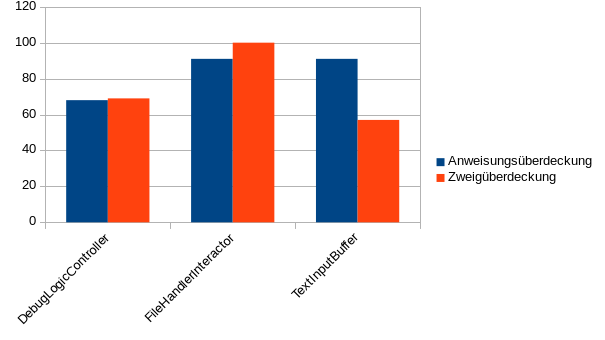
\includegraphics[width=0.8\textwidth]{ueberdeckung-kontrolle.png}
    \caption{Testüberdeckung der Teile von Control erreicht durch Komponententests, Integrationstests und Systemtests}\label{AbdeckungImInterpreter}
\end{figure}

\subsubsection{Testen Ladens von Konfigurationsdateien}
\textit{FileHandlerInteractor} ermöglicht dass Laden von Konfigurationsdateien mit der Methode \textit{applyConfiguration}.
Dabei wird nach Auslesen einer solchen Datei DIbugger in den Stand zurückversetzt, in dem DIbugger sich beim Speichern der Datei befand.
Um dies zu ermöglichen speichert \textit{FileHandlerInteractor} die in der Datei enthaltenen Daten im Modell DebugLogic, wie zum Beispiel die Zeilennummern von bedingten Breakpoints.
Außerdem wird die Präsentationskomponente \textit{dibugger.userinterface} dazu aufgefordert bestimmte Texte anzuzeigen wie zum Beispiel Programmtexte.
Insgesamt werden aus diesen beiden Paketen 10 verschiedene Methoden aufgerufen.
Unter Verwendung von Testhelfern (das sind Platzhalter oder Stellvertreter für andere Systemkomponenten des Systems) wurde getestet, ob Anzahl und Art dieser Funktionsaufrufe dem Sollverhalten entsprechen.
Das Sollverhalten ist in einem Sequenzdiagramm des Entwurfsdokumentes beschrieben, und wurde in der Implementierungsphase aus der Schnittstelle der Klasse für Konfigurationsdateien abgeleitet.
Eine Abweichen von diesem Verhalten wurde gefunden und ist in Abschnitt \ref{fehlerInControl} beschrieben.\\
(siehe \textit{test.control.FileHandlerInteractorTest, dibugger.debuglogic.debugger.ConfigurationFile})

\subsubsection{Beim Komponententest gefundene Fehler in Control}\label{fehlerInControl}
Beim Laden von Konfigurationsdateien mittels \textit{applyConfiguration} wurde die in der Datei enthaltene Einstellung für Schrittgröße eines Programmes nicht übernommen.\\
Der Fehler wurden beim Testen entdeckt (Testfall \textit{testApplyConfiguration\_valid} der Testklasse \textit{FileHandlerInteractorTest}).\\
Der Methodenaufruf zum Speichern der Schrittgrößeneinstellung erfolgt über eine andere Klasse (\textit{dibugger.controlDebugLogicControl}) und beim Aufruf wird eine Programmkennung mitübergeben.
Die übergebene Programmkennung muss aber vor Aufruf der Methode der Klasse (\textit{dibugger.control.DebugLogicController}) über eine andere Zugriffsmethode übergeben werden.
Dies wurde zur Fehlerbehebung umgesetzt.

Beim Laden von Konfigurationsdateien mittels \textit{applyConfiguration} wurden die in der Datei enthaltenen Watch-Expressions und bedingte Breakpoints mehrfach im Modell DebugLogic gespeichert.\\
Der Fehler wurden beim Testen entdeckt (Testfall \textit{testApplyConfiguration\_valid} der Testklasse \textit{FileHandlerInteractorTest}).\\
Ursache für den Fehler war, dass die Funktionsaufrufe zum Speichern innerhalb eines Schleifenrumpfes standen. 
Sie wurden zur Fehlerbehebung aus dem Schleifenrumpf entfernt.

\subsection{Filehandler}
\subsubsection{Klassenweite Tests}
Der Filehandler ist zuständig für das Laden von Dateien. Hier wurde darauf geachtet, dass die Klassen des Paketes \textit{filehandler.rdbf} ausgiebig getestet werden, da diese die Datenstruktur des \textit{Relational Dibugger Formats (RDBF)} repräsentieren und eine fehlerhafte Datenstruktur direkt zu einer fehlerhaften Datei führt.\\
Es wurde als Abdeckungskriterium die Anweisungsüberdeckung gewählt. Bei vorkommenden Verzweigungen handelt es sich in großen Teilen um von Java geforderte Fehlerbehandlung (beispielsweise Exception-Behandlung beim Einlesen einer nicht-existenten Datei, was die Benutzeroberfläche durch den FileChooser-Dialog bereits verhindert), weswegen die Zweigabdeckung für den Filehandler weniger relevant ist.

\subsubsection{Paketweite Tests}
Es wurde das korrekte Lesen und Schreiben von Dateien durch die im Paket enthaltenen \textit{Writer-} und \textit{Reader-}Klassen überprüft.
Da ein korrektes Lesen und Schreiben eine korrekte Datenstruktur impliziert, wurden die Klassen \textit{ConfigurationFile}, \textit{LanguageFile} und \textit{PropertiesFile} somit implizit getestet. Weitere implizit getestete Klassen sind \textit{RDBFFile} und die \textit{FileHandlerFacade}. Erstere enthält lediglich eine Variable und ihre Überklasse wurde getestet. Letztere reicht lediglich Arbeit an andere Klassen weiter.

\subsubsection{Im FileHandler gefundene Fehler}
Im \textit{FileHandler} gab es keine größeren Fehler. Lediglich zwei kleinere, namentlich einen \textit{Copy / Paste} Fehler und das Übersehen von negativen Zahlen in der RDBF-Grammatik.

\newpage
\section{Gesondertes Testen der Benutzeroberfläche}\label{gui}

\subsection{Übersicht über das Testen der Benutzeroberfläche}
Da automatisiertes Testen der Benutzeroberfläche sehr zeitaufwändig ist, wurde die Benutzeroberfläche des Dibuggers nach einem eigenen Testplan getestet. Dieser besteht zunächst aus sowohl dummem als auch intelligentem \textit{Monkey Testing}, um Schwächen oder Absturzpunkte der Benutzeroberfläche zu finden. \\
Anschließend wurde die Benutzeroberfläche von den Entwicklern hinsichtlich Nutzerfreundlichkeit betrachtet. Aufgrund der Gefahr, hier wichtige Kriterien zu übersehen, wird zusätzlich eine Benutzerstudie durchgeführt. \\
Außerdem wurden alle Funktionen der Benutzeroberfläche einzeln (z.B. jeder Button und Menüeintrag für sich) getestet, um diese Basisfunktionen dann in den Anwendungsfällen, welche im Pflichtenheft beschrieben wurden, zusammenzufassen. Die einzelnen Funktionen wurden hierbei in die Kriterien Gestaltung, Funktionalität und Performanz aufgeteilt.


\subsection{Monkey Testing}
Aus praktischen Gründen wurde das Monkey Testing manuell ausgeführt.
\subsubsection{Dummes Monkey Testing}
Unter \textit{dummem Monkey Testing} versteht man das Testen des Produktes ohne Wissen über das Produkt, die Gültigkeit oder Ungültigkeit der Eingabevariablen und  das Verhalten des Produkts. \\
Unter dummem Monkey Testing zeigte sich unser Produkt sehr stabil. So führte keine getestete, zufällige Kombination von Aktionen zu einem Absturz des Programms. 
\subsubsection{Intelligentes Monkey Testing}
Unter \textit{intelligentem Monkey Testing} versteht man das Testen des Produktes mit rudimentärem Wissen über das Produkt, Kenntnis des gegenwärtigen Zustandes, vergangener Zustände und  möglicher zukünftiger Zustände und Fähigkeiten des Systems. \\
Auch unter intelligentem Monkey Testing bestand das Produkt, nach Behebung zweier Fehler, die Tests. Zwischenzeitlich auftretende Fehler in den \textit{ExpressionPanels} und im Verändern der Größe dess gesamten Fensters führten zu einem Einfrieren der Benutzeroberfläche. Seit der Behebung dieser Fehler führte keine Kombination von Aktionen zum Absturz und Fehler die Auftraten wurden abgefangen und korrekt behandelt.

\subsection{Untersuchung der Nutzerfreundlichkeit}
Zur Verbessserung der Benutzerfreundlichkeit wurde zu den \textit{ExpressionPanels} jeweils ein +-Button hinzugefügt, um das Hinzufügen von Relationalen Ausdrücken intuitiver zu gestalten. Aufgrund der Funktionsweise der \textit{javax.swing.JTable} Komponente, muss zu jedem Zeitpunkt mindestens eine Expression in den Tabellen des \textit{WatchExpressionPanels} und des \textit{ConditionalBreakpointPanels} stehen. \\
Nach Auswertung der Benutzerstudie wurden außerdem Tooltips für die Laden- und Speicher-Buttons der \textit{ProgramPanels} hinzugefügt.

\subsection{Test der Grundfunktionen}
\subsubsection{Gestaltung}
\paragraph{Getestete Funktionen}
In diesem Bereich wurde die Anpassung des Produkts an die vom Benutzer gewählte Fenstergröße getestet. Außerdem wurden sämtliche PopUps auf ausreichende Größe überprüft.
Weitere Basisfunktionen im Bereich Gestaltung sind das korrekte Anzeigen der Scrollbalken, der hinzugefügten ProgramPanels und des Texts in den Textboxen.
\paragraph{Vorgenommene Änderungen}
Bei Untersuchung der Gestaltung der Benutzeroberfläche  fiel auf, dass sich ausschließlich die Größe des \textit{MainInterface} ändern lies, die Komponenten innerhalb jedoch bei einer festen Größe blieben. Außerdem verdeckte das rechte Control-Panel, welches die \textit{ExpressionPanels} und das \textit{CommandPanel} enthält, bei zu großer Fenstergröße die \textit{ProgramPanels} und versteckte bei zu kleiner Fenstergröße den Inhalt der \textit{ExpressionPanels}.\\
Das rechte Control-Panel bleibt nun bei einer festen Größe, um keinen Platz zu verschwenden. Bei Vergößern oder Verkleinern passt sich der Editor der ProgramPanels an die Größe des Fensters an.
\subsubsection{Funktionalität}
\paragraph{Getestete Funktionen}
\subparagraph{Menüs}
Es wurde getestet, ob die Menüeinträge und deren ActionListener valide sind, also ob die richtigen Optionen (zB verschiedene Sprachdateien) verfügbar sind, und richtig angewählt werden können.  \\
Zusätzlich wurden die Sprachdateien auf Vollständigkeit überprüft, und anschließend ob das Ändern der Sprache jederzeit möglich ist. \\
Die PopUps für Vorschläge wurden auf korrekte Funktionalität und Sprache überprüft, sowie die Menüeinträge für Vorschläge auf korrektes Aufrufen der jeweiligen PopUps. \\
Es wurde sichergestellt, dass vorgenommene Einstellungen im Einstellungsmenü nach Neustart des Produkts gleichbleiben.
\subparagraph{ProgramPanel}
Hinzufügen und Löschen bzw Zurücksetzen von ProgramPanels wurde in verschiedenen Reihenfolgen überprüft, um zusätzlich zu testen ob die Programmbezeichner korrekt berechnet werden. \\
Die Textfelder für Eingabevariablen und Schrittgröße wurden auf korrektes Weitergeben ihrer Daten geprüft. \\
Im Editorfeld, welches das jeweilige Programm enthält, waren folgende Funktionen zu testen:
\begin{itemize}
\item Hinzufügen, Löschen und Anzeige von (aktiven) Breakpoints an Zeilen im Text
\item Korrekte Zeilennummerierung bei Änderungen im Code
\item Markierbarkeit, Kopierbarkeit, Anzeige und Tab-Funktionalität im Text
\end{itemize}
Außerdem wurde die korrekte Returnvalue und das Anzeigen, Aus-und Einblenden von Variablen im Variableninspektor überprüft.
\subparagraph{Rechtes Control-Panel}
Das \textit{CommandPanel} wurde auf korrektes Ausgrauen der Buttons und richtige Übergabe von Benutzereingaben getestet. \\
Folgende Funktionalitäten wurden in den \textit{ExpressionPanels} überprüft:
\begin{itemize}
\item Anzeige der Auswertung
\item Übergabe der Expression
\item Hinzufügen und Löschen von Expressions
\item PopUps für Bereichsbindung
\end{itemize}
\paragraph{Vorgenommene Änderungen}
Es wurden fehlende Übersetzungen, wie zum Beispiel der Tooltip für \textit{StepOver}, zu allen Sprachdateien hinzugefügt. \\
Beim Speichern einer Konfigurationsdatei musste der Nutzer zunächst selbst die Dateiendung \textit{.rdbf} anhängen. Dies wurde geändert, sodass die korrekte Dateiendung automatisch angehängt wird, wenn nicht von Benutzer angegeben. \\ 
Beim Laden von Konfigurationsdateien trat aufgrund von vertauschten Parametern im Konstruktor der Fehler auf, dass der Programmcode selbst als Programmbezeichner benutzt wurde. Dies wurde korrigiert und Konfigurationsdateien lassen sich nun korrekt laden. \\
Es stellte sich während der Qualitätssicherungsphase heraus, dass im Editor stehender Text bei Markierung zum Teil verschwindet und erst wieder angezeigt wird, sobald der Benutzer mit der Maus außerhalb der \textit{javax.swing.JEditorPane}-Komponente klickt. Dieses Fehlverhalten ist darin begründet, dass für die Funktionalität der Breakpoints und Zeilennummerierung ein updaten der Komponente nötig ist. Wird währenddessen Text markiert, kann dieser aufgrund der Arbeitsweise des \textit{javax.swing.JEditorPane} nicht mehr korrekt dargestellt werden, bleibt aber bestehen. Somit stellt dieses Problem zwar ein Ärgernis dar, mindert aber nicht die Funktionalität des Produkts. \\ Obwohl die grobe Ursache des Problems gefunden wurde, konnte keine Möglichkeit gefunden werden, das Problem zu lösen ohne die Funktionalität der Zeilennummerierung oder der Breakpoints zu gefährden.
\subsubsection{Performanz der Elemente der Benutzeroberfläche}
\paragraph{Getestete Funktionen}
Während sämtlichen Tests der Benutzeroberfläche wurde darauf geachtet, ob es spürbare und störende Zeitverzögerungen bei Benutzung des Produkts gibt. Dies war nicht der Fall, jedoch kann sich in den Tests des Gesamtprodukts noch herausstellen, dass sich das Generieren des Traces, bei Betätigung des \textit{Debugmodus starten}-Buttons, unter ungünstigen Bedingungen verzögern kann.

\label{testszenarien}
\subsection{Testszenarien}
Bei den Testszenarien wurden die Anwendungsfälle AF10 bis AF60 aus dem Pflichtenheft getestet, indem die Anwendungsfälle aus den zuvor getesteten Grundfunktionen zusammengesetzt wurden. Diese wurden nach den vorangehenden Tests der Grundfunktionen manuell in der hier angegebenen Reihenfolge erfolgreich durchgeführt.
\begin{itemize} 
	\item[AF10] Hinzufügen von Programmen beinhaltet: 
	\begin{itemize}
		\item Menüeinträge sind vorhanden und anzeigbar
		\item Menüeintrag \textit{Programm hinzufügen} funktioniert
		\item PopUps funktionieren (um die Datei auszuwählen)
		\item Das ProgramPanel funktioniert mit all seinen Einzelkomponenten
	\end{itemize}
	\item[AF20] Ändern von Programmen beinhaltet:
	\begin{itemize}
		\item CommandPanel funktioniert
		\item Textfeld funktioniert (editierbar, kopierbar etc.)
		\item ProgramPanel funktioniert (für Änderungen an Eingaben etc.)
	\end{itemize}
	\item[AF30] Setzen von Breakpoints beinhaltet:
	\begin{itemize}
		\item Breakpoints lassen sich im ProgramPanel setzen, oder:
		\item ConditionalBreakpointPanel funktioniert
		\item PopUp für Bereichsbindung funktioniert, falls es ein bedingter Breakpoint war
	\end{itemize}
	\item[AF40] Hinzufügen von Watch-Expressions beinhaltet:
	\begin{itemize}
		\item WatchExpressionPanel funktioniert
		\item PopUp zur Bereichsbindung von WatchExpressions funktioniert
	\end{itemize}
	\item[AF50] Codes debuggen beinhaltet:
	\begin{itemize}
		\item Programm lässt sich über \textit{Programm hinzufügen} oder \textit{Programm öffnen} einbinden
		\item Breakpoints lassen sich setzen
		\item Watch-Expression und bedingte Breakpoints lassen sich hinzufügen und bearbeiten
		\item Der Text im Textfeld lässt sich ändern
		\item Der Debugmodus lässt sich starten
		\item Schritte, Einzelschritte, Continue etc. lassen sich ausführen
		\item Watch-Expression und bedingte Breakpoints werden richtig ausgewertet
		\item Der Rückgabewert wird richtig angezeigt
	\end{itemize}
	\item[AF60] Speichern eines Durchlaufs beinhaltet:
	\begin{itemize}
		\item Menüeinträge sind vorhanden
		\item Menüeinträge sind valide
		\item Konfigurationsdatei lässt sich speichern
		\item PopUp zum Speichern einer Konfigurationsdatei funktioniert
	\end{itemize}
\end{itemize}

\subsection{Benutzerstudie}\label{usertestimdoc}

\subsubsection{Testaufbau}

Im Pflichtenheft wurden bezüglich der Benutzeroberfläche ein besonderer Fokus auf Verständlichkeit, Übersichtlichkeit und Erlernbarkeit gelegt. Dem wurde mit einem gesonderten Nutzertest Rechnung getragen. \\
Im Anhang findet sich unter Punkt \ref{usertest} das Protokoll für den Versuchsaufbau. Dieser besteht aus zwei Teilen: Zunächst setzt die Testperson mit Hilfe des DIbuggers mehrere praktische Aufgaben um. Geprüft werden die in Tabelle \ref{testfaelle} aufgelisteten Grundfunktionalitäten des DIbuggers. Zunächst soll versucht werden, die Aufgabe ohne Hilfestellung zu lösen. Schlägt dies fehl, darf das Nutzermanual zu Rate gezogen werden (und wird somit ebenfalls auf Verständlichkeit geprüft). Die Testleitung soll nur die letzte Instanz sein. \\
Die Testperson wird dabei von der Versuchsleitung zum lauten Denken angehalten. So können nicht nur Probleme erkannt werden, die die Ausführung einer Aufgabe für die Versuchsperson unmöglich machen, sondern auch Programmeigenschaften, die die Ausführung verzögern oder umständlich machen. \\
Die zwei Programme, die von den Nutzern untersucht werden sollen, sind ebenfalls im Anhang, unter Punkt \ref{code} zu finden.
Im zweiten Teil der Untersuchung füllt die Versuchsperson einen zweiseitigen Fragebogen aus, der aus statistischen und offenen Fragen besteht.

\begin{table}
\begin{tabular}{l||c}
   	Aufgabe & Getestetes DIbugger-Konzept \\
	\hline
	\hline
	1 & Nutzen der Menüleiste, Anzeigen der Hilfe\\
	2 & Nutzen der Menüleiste, Ändern der Sprache\\
	3 & Hinzufügen eines neuen Programmfensters \\
	4 & Löschen eines Programmfensters \\
	5 & einfache Wlang-Syntax, Fehlermeldungen, Variablenanzeige, Steps \\
	6 & Anordnung und Aufrufen von Funktionen, Fehlermeldungen, Speichern \\
	7 & Laden einer Konfiguration, Bedingte Breakpoints, Watch-Expressions \\
	8 & Watch-Expression-Menüs


\end{tabular}
\label{testfaelle}
\caption{Hintergrund der Aufgaben im Praxisteil}
\end{table}



\subsubsection{Auswertung}

\subsubsection{Auswertung}
Getestet wurden acht Testpersonen (alle männlich, 20-27 Jahre alt, Studenten mit Haupt- oder Nebenfach Informatik).
Im Allgemeinen lässt sich sagen, dass das Nutzerhandbuch und die Übersichtlichkeit der Benutzeroberfläche als hilfreich und nutzerfreundlich empfunden wurden. Probleme ergaben sich vor allem beim Verständnis von speziellen Konzepten des \textit{DIBuggers}, wie zum Beispiel von Watch-Expressions, und beim Erlernen der WLang-Syntax. Diesen Problemen wurde mit der Verfeinerung von Exceptions und Änderungen an der Benutzeroberfläche sowie dem Nutzerhandbuch entgegengewirkt.\\
Im Folgenden werden die Ergebnisse und ihre Verbesserung im Detail erklärt:

\paragraph{Nutzen der Menüleiste (Aufgaben 1-3)}
Im Praxisteil wurden die Aufgaben 1 bis 3 (siehe Tabelle \ref{testfaelle}) jeweils in wenigen Sekunden und fehlerfrei ausgeführt, d.h. die Testpersonen konnten das Nutzerhandbuch finden, die Sprache umstellen und ein neues Fenster hinzufügen.\\
Auch im Fragebogen wurden das Nutzerhandbuch und die Übersichtlichkeit der Benutzeroberfläche durchweg als hilfreich und nutzerfreundlich bewertet.\\
Dies könnte darauf zurückzuführen sein, dass die Menüleiste sich in ihrer Struktur an Konventionen orientiert, die den Nutzern bekannt sind.

\paragraph{Löschen eines Programmfensters (Aufgabe 4)}
Die Testpersonen fanden den Entfernen-Knopf (mit einem roten X-Symbol versehen) über den jeweiligen Programmfenstern zügig und konnten das Programm löschen. Auch dies könnte auf Konventionen zurückzuführen sein. \\Allerdings wurde angeregt, auch für die mit Bildern belegten Knöpfe Tooltips zur Rückversicherung einzusetzen.\\\\
Vorgenommene Verbesserung:\\
Es wurden entsprechend Tooltips bei den Knöpfen eingefügt.

\paragraph{Wlang-Syntax (Aufgaben 5-6)}
Im Praxisteil gelang es den Versuchspersonen trotz des Beispieltextes in den Programmfenstern nur mit erhöhtem Zeitaufwand und mehreren Anläufen, ein korrektes WLang-Programm zu schreiben. Das Nutzermanual musste jedes Mal zu Rate gezogen werden, half aber beim Finden des Fehlers.\\
Auch im Fragebogen wurden zu diesem Punkt die meisten Anmerkungen gemacht. Die Nutzer wünschten sich vor allem konkretere Hinweise auf Fehler, am liebsten mit Syntax-Highlighting. \\
Eine Erklärung für die Schwierigkeiten könnte sein, dass WLang einigen Erwartungen an übliche Programmiersprachen, wie zum Beispiel Java, nicht entspricht. Des Weiteren sind die Nutzer vermutlich die Hilfe von Entwicklungsumgebungen gewohnt, die die Fehlerfindung erleichtern. Außerdem muss man uns Entwicklern eine gewisse Betriebsblindheit unterstellen, denn natürlich ist die Fehlersuche leichter, wenn man die Sprache selbst definiert hat.\\\\
Vorgenommene Verbesserung:\\
Die Exception-Behandlung des Antlr-Pakets wurde so angepasst, dass sie nicht nur die Zeilennummer, sondern auch das Vorkommen eines Fehlers innerhalb der Zeile angibt.\\
(siehe \textit{dibugger.debuglogic.antlrparser.ActuallyHelpfulErrorListener})\\
Des Weiteren wurde das Nutzerhandbuch an mehreren Stellen ergänzt. Unter anderem wurde der Abschnitt zu üblichen Fehlern erweitert.
%
%
%\paragraph{Laden einer Konfiguration (Aufgabe 7)}
%In Aufgabe 6 sollten die Testpersonen eine vorbereitete \textit{DIbugger}-Konfiguration in den \textit{DIbugger} laden. Obwohl diese Aufgabe ohne Nutzung des Manuals erledigt werden konnte und die Testpersonen schnell den richtigen Menü-Unterpunkt aufriefen, kam es doch zu Verzögerungen, weil der Menüpunkt \enquote{Konfiguration laden} und nicht \enquote{Datei laden} heißt.\\
%Dieses Hindernis ist ein weiteres Beispiel für Betriebsblindheit während der Entwicklung, denn Nutzern ist eine Konfiguration ohne gesonderte Erklärung kein Begriff.\\\\
%Vorgenommene Verbesserung:\\
%Der entsprechende Menüpunkt wurde umbenannt.


\paragraph{Nutzen von Bedingten Breakpoints und Watch-Expressions (Aufgabe 7)}
Im Praxisteil wurden Bedingte Breakpoints und Watch-Expressions nach kurzem Nachdenken und Explorieren oder nach Nachlesen im Benutzerhandbuch erfolgreich genutzt.\\
Dazu scheinbar widersprüchlich wurde von einigen Nutzern im Fragebogen der Wunsch nach einer besseren Einführung in diese beiden \textit{DIbugger}-Konzepte geäußert.\\
Eine tatsächliche Schwierigkeit bereitete das Verständnis der Auswertung von Bedingten Breakpoints.
\\
Es ist verständlich, dass Nutzern ohne Vorkenntnis Bedingte Breakpoints und Watch-Expressions kein Begriff sind. Dass diese Funktionen trotzdem zügig und mit weitgehend korrekter Syntax genutzt wurden, liegt wohl an den Beispielen, die beim Programmstart standardmäßig angezeigt werden. Möglich wäre auch, dass die Versuchspersonen bei der Aufgabenerfüllung davon ausgingen, dass sie die in vorigen Aufgaben noch nicht betrachteten Panels der Benutzeroberfläche nutzen sollten.\\\\
Vorgenommene Verbesserung:\\
Da die Nutzung von Bedingten Breakpoints und Watch-Expressions im Allgemeinen zügig und erfolgreich war, wurde aus Gründen der Übersichtlichkeit (die ja ebenfalls eine nicht-funktionale Anforderung der Benutzeroberfläche darstellt) darauf verzichtet, in der Benutzeroberfläche direkt eine Erklärung zu bieten. Stattdessen wurde das Manual erweitert.

\paragraph{Nicht explizit erwähnte Verbesserungen}
Wenn eine einzelne Person ein Problem mit der Benutzung des \textit{DIbuggers} hatte, die ihre Ursache tatsächlich im Produkt und nicht zum Beispiel einer fehlenden Sehhilfe hatte, wurde das Nutzermanual entsprechend erweitert oder verbessert.

\paragraph{Weitere mögliche Verbesserungen}
Viele weitere Änderungen sind denkbar. So könnten noch mehr Exceptions eingeführt werden, um die Fehlerbehandlung für den Nutzer transparenter zu machen, insbesondere bei der WLang-Syntax. Weitere Buttons könnten für ein schnelles Hinzufügen neuer Programmfenster eingefügt werden. Ein interaktives Tutorial könnte eine schnelle Einführung in das Produkt geben. Auch ein Syntax-Highlighting denkbar. 










\newpage
\section{Testen des Gesamtprodukts}\label{gesamthwsw}

\subsubsection{Produktfunktionen}
Viele Anforderungen an das Produkt wurden bereits mit den Testszenarien der Benutzeroberfläche (\ref{testszenarien}) getestet, die aus den Anwendungsfällen aus dem Pflichtenheft generiert wurden, um die graphische Benutzeroberfläche zu testen.
\\
 \\
So wurden die zum Debugging-Mechanismus gehörenden funktionalen Anforderungen (FA10-30, 50-130, 180-215, 240, 310) durch das Testszenario zum Anwendungsfall 50 ("Codes debuggen") getestet.
Das Einbinden von Programmen (FA170) wurde durch das Testszenario zu AF10 ("Hinzufügen von Programmen") abgedeckt, das Schreiben und Kopieren von Texten in Textfenster (FA150 und FA160) wurde durch das Testszenario zu AF20("Ändern von Programmen" und das Speichern der Konfigurationsdateien durch das Testszenario zu AF60 ("Speichern eines Durchlaufs") abgedeckt.
\\
 \\
Die Funktionalen Anforderungen zu Schrittgrößen (FA40) und Vorschlägen (FA220, 270, 280, 300) wurde durch folgendes Szenario abgedeckt: \\
\textbf{Szenario 1}: Zu den vorhandenen Beispielprogrammen gibt der Benutzer jeweils von 1 abweichende, unterschiedliche Schrittgrößen ein. Dann führt er den Debuglauf aus, um diesen dann anzuhalten und sich Schrittgrößen für die beiden Programme vorschlagen zu lassen und diese zu übernehmen. Dann lässt er sich jeweils zwei Watch-Expressions und bedingte Breakpoints vorschlagen und startet den Debuglauf erneut. Der Debuglauf wird bis zum Ende durchgeführt und dann beendet.
\\
 \\
Die Funktionale Anforderung, dass man mehr als zwei Programme gleichzeitig debuggen kann, wird durch folgendes Szenario abgedeckt: 
\\
\textbf{Szenario 2}: Der Benutzer fügt zu den beiden Beispielprogrammen zwei weitere Programme hinzu, welche er selbst geschrieben hat (in unserem Test noch einmal die selben Programme). Dann führt er für alle vier Programme das Testszenario zu AF50 aus.
\\
 \\
Die Anforderungen zu den Produktdaten bezüglich der Konfigurationsdatei wurden ebenfalls mittels des Testszenarios zu AF50 getestet. Die Sprachdateien wurden während des Testens der graphischen Benutzeroberfläche getestet. Für die Einstellungsdatei wurde ein weiteres Szenario entwickelt: \\
\textbf{Szenario 3}: Der Benutzer führt AF50 aus, ändert dann die Sprache, schließt das Produkt und öffnet es dann anschließend erneut. \\
 \\
Die Anforderungen zu den Produktleistungen wurden ebenfalls größtenteils durch das Testen der graphischen Benutzeroberfläche abgedeckt: Der Punkt Performanz der Benutzeroberfläche beinhaltet auch das Zeitverhalten des Produkts (PL10) und das Monkey Testing deckt die Fehlertoleranz (PL30) ab. Zur Genauigkeitsüberprüfung dienten die JUnit-Tests zu den TermValues die überprüft haben, ob die arithmetischen Operationen wie in Java ausgeführt werden. \\
 \\
Die Benutzerfreundlichkeit (NA50) wurde durch die Nutzerstudie überprüft. 

\subsubsection{Globale Testfälle des Pflichtenhefts} %TODO
Die globalen Testfälle aus dem Pflichtenheft T10 bis T380 wurden, bis auf die Ausnahmen T60, T100 und T360, welche zu keiner umgesetzten funktionalen Anforderung gehören, manuell ausgeführt und getestet. Bei wenigen Testfällen gab es dabei kleine Abänderungen, da die zugehörigen Funktionen anders implementiert wurden als im Pflichtenheft noch angenommen. \\
Die Änderungen sind: \\
\begin{itemize}
	\item in manchen Testfällen wurden die Bezeichner von Aktionen verändert (z.B. T20, T40)
	\item in T70 wird ein Breakpoint nun gelöscht indem man ihn mit Doppelklick entfernt statt mit einem einfachen Klick
	\item  in T190 wird der Rückgabewert nicht erst nach Ende des Debuglaufs angezeigt sondern sofort nach Beginn
	\item in T260 kann der Benutzer eine Bereichsbindung nur löschen, indem er als Bereich das gesamte Programm eingibt
	\item in T270 und T330 kann man eine Bereichsbindung nur anzeigen, indem man auf das Optionenfeld der Watch-Expression klickt und \enquote{Bereichsbindung ändern} auswählt
	\item in T370 eine Variable wird durch Auswählen und Rechtsklick entfernt und alle Variablen werden wieder angezeigt, wenn der Button \enquote{Ausgeblendete Variablen anzeigen} betätigt wird
\end{itemize}

\subsection{Weitere Testfälle}

\subsubsection{Belastungstests} %TODO
\label{stress}
Auch Randfälle des Einsetzens wurden über Unit-Tests oder über die Benutzeroberfläche getestet: 
\begin{itemize}
%\item Tiefe Rekursion (Ackermann) (zum Zeitpunkt der Vorabgabe noch nicht fertig gestellt)
\item Endlosschleifen: Das Produkt benachrichtigt den Benutzer über das Überschreiten der von ihm ausgewählten maximalen Anzahl der Iterationen und das Auftreten im Programm und beendet den Debugvorgang.
\item falsche Nutzereingaben: Das Produkt benachrichtigt den Benutzer über falsche Syntax und beendet den Debugvorgang. Syntaktisch falsche \textit{Relational Expressions} werden zu \enquote{?} ausgewertet.
\item keine Nutzereingaben
\item n Programme gleichzeitig debuggen
\item leere Fenster: Gibt der Benutzer kein Programm in einem seiner \textit{ProgramPanels} ein, so benachrichtigt das Produkt den Benutzer über falsche Syntax und beendet den Debugvorgang.
\item Dateien laden, die nicht dem RDBF-Format entsprechen: Das Produkt benachrichtigt den Benutzer darüber, dass die von ihm ausgewählte Datei invalide ist.
\item ...

\end{itemize}

\subsection{Test auf verschiedener Hard- und Software}

Das Produkt wurde sowohl auf Windows (7 und 10), als auch auf Linux (Ubuntu 17.04 64bit und KDE Neon 5.11.3 64bit) erfolgreich getestet, indem alle JUni-Tests der einzelnen Pakete, die Tests der graphischen Benutzeroberfläche und die in diesem Kapitel aufgeführten Tests des Gesamtprodukts auf den unterschiedlichen Rechnern durchgeführt wurden.

Die Tests wurde auf Rechnern mit folgender Hardware erfolgreich durchgeführt: \\ \\
\begin{tabular}{l||l|l}
   	 & Prozessor & RAM \\
	\hline
	\hline
	Rechner 1 & AMD Phenom II X4 B50 4K 4T @3.5Ghz & 10GB DDR3 \\
	Rechner 2 & Intel Core i3-380M 2K 4T @2.5Ghz & 8GB DDR3 \\
	Rechner 3 & Intel Core i5-7200U @3.1Ghz & 8GB DDR3 \\
	Rechner 4 & Intel Core i7-7500U @2.7Ghz & 16GB DDR4\\
\end{tabular}


\subsection{Untersuchung von Laufzeit und Speicherverbrauch}
(Diese Untersuchung ist geplant für diese Woche.)



\newpage
\section{Fazit}
%TODO



\newpage

\printglossary[style=altlist, toctitle=Glossar]
\newpage

\section{Anhang}
%getestete Programme
\subsection{Testprogramme für die Nutzerstudie}\label{code}
\textbf{Programm A:}
\begin{verbatim}
int main (int n) {
	int a = 1;
	int b = 0;
	int c = 34723;
	while (a < 2*n) {
		b = b + a;
		a = a + 2;
		c = c*a-b;
	}
	return b;
}
\end{verbatim}

\textbf{Programm B:}
\begin{verbatim}
int foo(int k) {
	int i = 0;
	int d = 0;
	while(i < k) {
	i = i +1;
	d = d + k;
}
return d;
}
int main (int k) {

	int a = 0;
	a = foo(k);
	return a;
}
\end{verbatim}

\subsection{Testprotokoll für die Nutzerstudie}\label{usertest}
%Testprotokoll

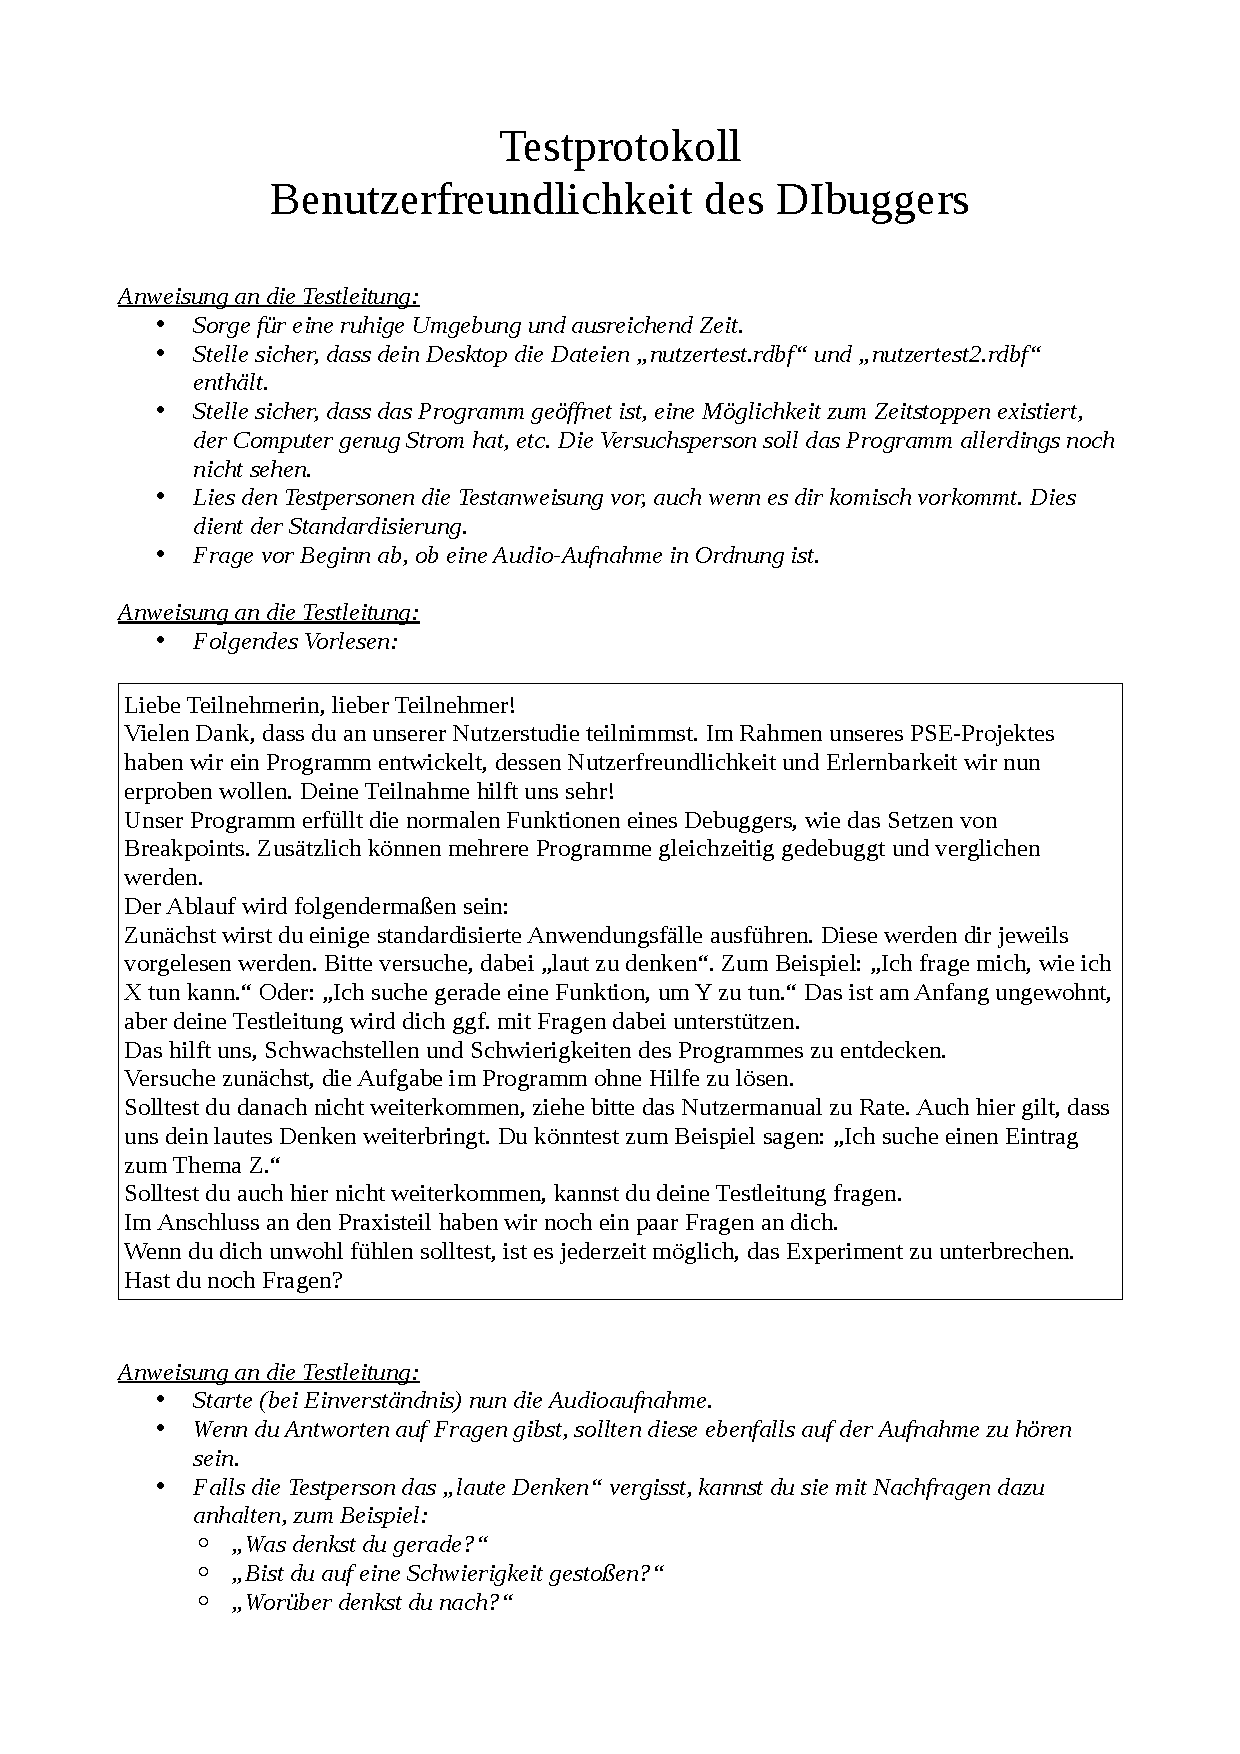
\includepdf[pages={1-},scale=0.75]{UsabilitytestDebugger.pdf}

\end{document}
